\documentclass[a4paper]{article}
\usepackage[utf8]{inputenc}

%_______________________________________________________________
%                    Packages needed:
%_______________________________________________________________
\usepackage{tikz, adjustbox}
\usepackage[most]{tcolorbox}
\usepackage{xcolor}
\usepackage{wrapfig}
\newcommand*{\plogo}{\fbox{$\mathcal{PL}$}} % Generic dummy publisher logo
\usepackage[utf8]{inputenc} % Required for inputting international characters
\usepackage[T1]{fontenc} % Output font encoding for international characters
\usepackage{stix} % Use the STIX fonts
\usepackage[utf8]{inputenc}
\usepackage{xcolor}
\usepackage[explicit]{titlesec}
\usepackage{soul}
\usepackage[a4paper, margin=1in]{geometry}

%................................................................
%
%           Defining colors for sticky notes:
%_______________________________________________________________
% Yellow:
\definecolor{BgYellow}{HTML}{FFF59C}
\definecolor{FrameYellow}{HTML}{F7A600}
% Pink:
\definecolor{BgPink}{HTML}{EF6FA7}
\definecolor{FramePink}{HTML}{E5446E}
% Green:
\definecolor{BgGreen}{HTML}{C7D92D}
\definecolor{FrameGreen}{HTML}{89B23B}
% Blue:
\definecolor{BgBlue}{HTML}{45BEE9}
\definecolor{FrameBlue}{HTML}{31A8C9}
% White:
\definecolor{BgWhite}{HTML}{D8D8D8}
\definecolor{FrameWhite}{HTML}{7F7F7F}
% Brown:
\definecolor{BgBrown}{HTML}{8E7A45}
\definecolor{FrameBrown}{HTML}{6B5B32}
%................................................................
%
%                   Dummy text package:
%_______________________________________________________________
\usepackage{lipsum}
%................................................................
%
%                   NB command:
%_______________________________________________________________
\usepackage{contour}
\newcommand{\NB}{\contour{black}{\textbf{{\large\sffamily\color{red}NB}}}\textbf{\large\sffamily: }}
%................................................................
%
%               Defining Sticky note boxes:
%_______________________________________________________________
% Yellow Sticky Note (YStkyNote):
\newtcolorbox{YStkyNote}[1][]{%
    enhanced,
    before skip=2mm,after skip=2mm, 
    width=0.4\textwidth, % width of the sticky note
    boxrule=0.2mm,
    colback=BgYellow, colframe=FrameYellow, % Colors
    attach boxed title to top left={xshift=0cm,yshift*=0mm-\tcboxedtitleheight},
    varwidth boxed title*=-3cm,
    % The titlebox:
    boxed title style={frame code={%
        \path[left color=FrameYellow,right color=FrameYellow,
        middle color=FrameYellow]
        ([xshift=-0mm]frame.north west) -- ([xshift=0mm]frame.north east)
        [rounded corners=0mm]-- ([xshift=0mm,yshift=0mm]frame.north east)
        -- (frame.south east) -- (frame.south west)
        -- ([xshift=0mm,yshift=0mm]frame.north west)
        [sharp corners]-- cycle;
        },interior engine=empty,
    },
    sharp corners,rounded corners=southeast,arc is angular,arc=3mm,
    % The "folded paper" in the bottom right corner:
    underlay={%
        \path[fill=BgYellow!80!black] ([yshift=3mm]interior.south east)--++(-0.4,-0.1)--++(0.1,-0.2);
        \path[draw=FrameYellow,shorten <=-0.05mm,shorten >=-0.05mm,color=FrameYellow] ([yshift=3mm]interior.south east)--++(-0.4,-0.1)--++(0.1,-0.2);
        },
    drop fuzzy shadow, % Shadow
    fonttitle=\bfseries, 
    title={#1}
}
% Pink Sticky Note (PStkyNote):
\newtcolorbox{PStkyNote}[1][]{%
    enhanced,
    before skip=2mm,after skip=2mm, 
    width=0.4\textwidth, % width of the sticky note
    boxrule=0.2mm, 
    colback=BgPink, colframe=FramePink, % Colors
    attach boxed title to top left={xshift=0cm,yshift*=0mm-\tcboxedtitleheight},
    varwidth boxed title*=-3cm,
    % The titlebox:
    boxed title style={frame code={%
        \path[left color=FramePink,right color=FramePink,
        middle color=FramePink]
        ([xshift=-0mm]frame.north west) -- ([xshift=0mm]frame.north east)
        [rounded corners=0mm]-- ([xshift=0mm,yshift=0mm]frame.north east)
        -- (frame.south east) -- (frame.south west)
        -- ([xshift=0mm,yshift=0mm]frame.north west)
        [sharp corners]-- cycle;
        },interior engine=empty,
    },
    sharp corners,rounded corners=southeast,arc is angular,arc=3mm,
    % The "folded paper" in the bottom right corner:
    underlay={%
        \path[fill=BgPink!80!black] ([yshift=3mm]interior.south east)--++(-0.4,-0.1)--++(0.1,-0.2);
        \path[draw=FramePink,shorten <=-0.05mm,shorten >=-0.05mm,color=FramePink] ([yshift=3mm]interior.south east)--++(-0.4,-0.1)--++(0.1,-0.2);
        },
    drop fuzzy shadow, % Shadow
    fonttitle=\bfseries, 
    title={#1}
}
% Green Sticky Note (GStkyNote):
\newtcolorbox{GStkyNote}[1][]{%
    enhanced,
    before skip=2mm,after skip=2mm, 
    width=0.4\textwidth, % width of the sticky note
    boxrule=0.2mm,
    colback=BgGreen, colframe=FrameGreen, % Colors
    attach boxed title to top left={xshift=0cm,yshift*=0mm-\tcboxedtitleheight},
    varwidth boxed title*=-3cm,
    % The titlebox:
    boxed title style={frame code={%
        \path[left color=FrameGreen,right color=FrameGreen,
        middle color=FrameGreen]
        ([xshift=-0mm]frame.north west) -- ([xshift=0mm]frame.north east)
        [rounded corners=0mm]-- ([xshift=0mm,yshift=0mm]frame.north east)
        -- (frame.south east) -- (frame.south west)
        -- ([xshift=0mm,yshift=0mm]frame.north west)
        [sharp corners]-- cycle;
        },interior engine=empty,
    },
    sharp corners,rounded corners=southeast,arc is angular,arc=3mm,
    % The "folded paper" in the bottom right corner:
    underlay={%
        \path[fill=BgGreen!80!black] ([yshift=3mm]interior.south east)--++(-0.4,-0.1)--++(0.1,-0.2);
        \path[draw=FrameGreen,shorten <=-0.05mm,shorten >=-0.05mm,color=FrameGreen] ([yshift=3mm]interior.south east)--++(-0.4,-0.1)--++(0.1,-0.2);
        },
    drop fuzzy shadow, % Shadow
    fonttitle=\bfseries, 
    title={#1}
}
% Blue Sticky Note (BStkyNote):
\newtcolorbox{BStkyNote}[1][]{%
    enhanced,
    before skip=2mm,after skip=2mm, 
    width=0.4\textwidth, % width of the sticky note
    boxrule=0.2mm,
    colback=BgBlue, colframe=FrameBlue, % Colors
    attach boxed title to top left={xshift=0cm,yshift*=0mm-\tcboxedtitleheight},
    varwidth boxed title*=-3cm,
    % The titlebox:
    boxed title style={frame code={%
        \path[left color=FrameBlue,right color=FrameBlue,
        middle color=FrameBlue]
        ([xshift=-0mm]frame.north west) -- ([xshift=0mm]frame.north east)
        [rounded corners=0mm]-- ([xshift=0mm,yshift=0mm]frame.north east)
        -- (frame.south east) -- (frame.south west)
        -- ([xshift=0mm,yshift=0mm]frame.north west)
        [sharp corners]-- cycle;
        },interior engine=empty,
    },
    sharp corners,rounded corners=southeast,arc is angular,arc=3mm,
    % The "folded paper" in the bottom right corner:
    underlay={%
        \path[fill=BgBlue!80!black] ([yshift=3mm]interior.south east)--++(-0.4,-0.1)--++(0.1,-0.2);
        \path[draw=FrameBlue,shorten <=-0.05mm,shorten >=-0.05mm,color=FrameBlue] ([yshift=3mm]interior.south east)--++(-0.4,-0.1)--++(0.1,-0.2);
        },
    drop fuzzy shadow, % Shadow
    fonttitle=\bfseries, 
    title={#1}
}
% White Sticky Note (WStkyNote):
\newtcolorbox{WStkyNote}[1][]{%
    enhanced,
    before skip=2mm,after skip=2mm, 
    width=0.4\textwidth, % width of the sticky note
    boxrule=0.2mm,
    colback=BgWhite, colframe=FrameWhite, % Colors
    attach boxed title to top left={xshift=0cm,yshift*=0mm-\tcboxedtitleheight},
    varwidth boxed title*=-3cm,
    % The titlebox:
    boxed title style={frame code={%
        \path[left color=FrameWhite,right color=FrameWhite,
        middle color=FrameWhite]
        ([xshift=-0mm]frame.north west) -- ([xshift=0mm]frame.north east)
        [rounded corners=0mm]-- ([xshift=0mm,yshift=0mm]frame.north east)
        -- (frame.south east) -- (frame.south west)
        -- ([xshift=0mm,yshift=0mm]frame.north west)
        [sharp corners]-- cycle;
        },interior engine=empty,
    },
    sharp corners,rounded corners=southeast,arc is angular,arc=3mm,
    % The "folded paper" in the bottom right corner:
    underlay={%
        \path[fill=BgWhite!80!black] ([yshift=3mm]interior.south east)--++(-0.4,-0.1)--++(0.1,-0.2);
        \path[draw=FrameWhite,shorten <=-0.05mm,shorten >=-0.05mm,color=FrameWhite] ([yshift=3mm]interior.south east)--++(-0.4,-0.1)--++(0.1,-0.2);
        },
    drop fuzzy shadow, % Shadow
    fonttitle=\bfseries, 
    title={#1}
}
% Brown Sticky Note (BrStkyNote):
\newtcolorbox{BrStkyNote}[1][]{%
    enhanced,
    before skip=2mm,after skip=2mm, 
    width=0.4\textwidth, % width of the sticky note
    boxrule=0.2mm,
    colback=BgBrown, colframe=FrameBrown, % Colors
    attach boxed title to top left={xshift=0cm,yshift*=0mm-\tcboxedtitleheight},
    varwidth boxed title*=-3cm,
    % The titlebox:
    boxed title style={frame code={%
        \path[left color=FrameBrown,right color=FrameBrown,
        middle color=FrameBrown]
        ([xshift=-0mm]frame.north west) -- ([xshift=0mm]frame.north east)
        [rounded corners=0mm]-- ([xshift=0mm,yshift=0mm]frame.north east)
        -- (frame.south east) -- (frame.south west)
        -- ([xshift=0mm,yshift=0mm]frame.north west)
        [sharp corners]-- cycle;
        },interior engine=empty,
    },
    sharp corners,rounded corners=southeast,arc is angular,arc=3mm,
    % The "folded paper" in the bottom right corner:
    underlay={%
        \path[fill=BgBrown!80!black] ([yshift=3mm]interior.south east)--++(-0.4,-0.1)--++(0.1,-0.2);
        \path[draw=FrameBrown,shorten <=-0.05mm,shorten >=-0.05mm,color=FrameBrown] ([yshift=3mm]interior.south east)--++(-0.4,-0.1)--++(0.1,-0.2);
        },
    drop fuzzy shadow, % Shadow
    fonttitle=\bfseries, 
    title={#1}
}

% 
\definecolor{titleblue}{HTML}{2A202C}

\newbox\TitleUnderlineTestBox
\newcommand*\TitleUnderline[1]
  {%
    \bgroup
    \setbox\TitleUnderlineTestBox\hbox{\colorbox{titleblue}\strut}%
    \setul{\dimexpr\dp\TitleUnderlineTestBox-.3ex\relax}{.3ex}%
    \ul{#1}%
    \egroup
  }
\newcommand*\SectionNumberBox[1]
  {%
    \colorbox{titleblue}
      {%
        \makebox[2.5em][c]
          {%
            \color{white}%
            \strut
            \csname the#1\endcsname
          }%
      }%
    \TitleUnderline{\ \ \ }%
  }
\titleformat{\section}
  {\Large\bfseries\sffamily\color{titleblue}}
  {\SectionNumberBox{section}}
  {0pt}
  {\TitleUnderline{#1}}
\titleformat{\subsection}
  {\large\bfseries\sffamily\color{titleblue}}
  {\SectionNumberBox{subsection}}
  {0pt}
  {\TitleUnderline{#1}}

  \usepackage{pgfplots}


\begin{document}
    \begin{titlepage}
        \raggedleft
        \rule{1pt}{\textheight}
        \hspace{0.05\textwidth}
        \parbox[b]{0.75\textwidth}{
            {\Huge\bfseries \textcolor[HTML]{2A202C}{Machine Learning}\\[0.5\baselineskip] \textcolor[HTML]{2A202C}{Specialization}}\\[2\baselineskip]
            {\large\textit{\textcolor[HTML]{2A202C}{Course Notes}}}\\[4\baselineskip]
            {\Large\textsc{\textcolor[HTML]{2A202C}{Jesus Cardenaz}}}
            
            \vspace{0.5\textheight}
        }
    \end{titlepage}

    \setlength{\parindent}{0pt}
    \setlength{\parskip}{5pt}


    \section{Supervised Vs. Unsupervised Machine Learning}
    \subsection*{What is Machine Learning?}
    "Machine Learning is the field of study that gives computers the ability to learn without being explicitly programmed." Arthur Samuel (1959)

    The two main types of Machine Learning are Supervised Learning and Unsupervised Learning. Supervised Learning, being the most widely used, is used in many real-world applications and has seen the most rapid advancements.

    Arthur Samuel's checkers playing program is a historical example of a learning algorithm.

    \subsection*{What is Supervised Learning}
    In Supervised Learning, algorithms learn input to output mappings from provided examples. The input and correct output (x and y) are provided to the learning algorithm, and by seeing these correct pairs, it learns to predict the output from the given input.

    This method of learning is used in spam filters, speech recognition, machine translation, online advertising, self-driving cars, and product inspection in manufacturing

    \subsubsection*{Most Common Types of Supervised Learning:}
    \begin{itemize}
        \item Classification: Predicts categorical outputs from a limited set of possibilities.
        \item Regression: Predicts numerical outputs from infinite possibilities.
    \end{itemize}

    \begin{center}
        \begin{YStkyNote}[Note 1]
            Classification differs from regression in that it does not predict all possible numbers in between categories
        \end{YStkyNote}
    \end{center}

    \paragraph*{Classification} Classification is a type of supervised learning where the output of the variable is categorical. i.e, it belongs to a specific finite set of categories or classes. The model is trained to predict the class of the given input data. Common classification algorithms include:
    \begin{itemize}
        \item Logistic Regression
        \item K-nearest Neighbors
        \item Support Vector Machines
        \item Decision Trees
        \item Random Forests
    \end{itemize}

    \paragraph*{Regression} Regression is another type of supervised learning where the output variable is continuous or numerical. The model learns to predict a value on the input data. Common regression algorithms include:
    \begin{itemize}
        \item Linear Regression
        \item Polynomial Regression
        \item Decision Trees 
        \item Random Forest 
        \item Support Vector Regression
    \end{itemize}    
    
    In addition to classification and regression, there are other types of supervised learning that cater to more specific needs: 
    \begin{itemize}
        \item Multi-label Classification.
        \item Multivariate Regression.
        \item Ordinal Regression (Ranking Learning).
        \item Time Series Prediction.
    \end{itemize}

    \subsection*{What is Unsupervised Learning?}
    Unsupervised learning is another type of machine learning where we provide the algorithm with data that isn't linked with any output labels. The algorithm's task is to identify patterns or structures in the data.

    A specific form of unsupervised learning is a clustering algorithm, used for instance in Google News to group related stories.

    \begin{center}
        \begin{YStkyNote}[Note]
                Unsupervised Learning involves identifying patterns and structures in data without any pre-existing labels.
        \end{YStkyNote}
    \end{center}
    
    \paragraph*{Clustering}
    Clustering is a specific type of unsupervised learning where the algorithm groups related data together. This technique can be used in many applications, such as news grouping, genetic data classification, and customer segmentation.

    \paragraph*{Anomaly Detection}
    An unsupervised learning technique that is used to detect unusual events in the data, which could potentially be signs of fraudulent activity or other abnormalities.

    \paragraph*{Dimensionality Reduction}
    Reduces a large dataset into a smaller one while retaining as much important information as possible.
    
    \subsection*{Linear Regression Model}

    \paragraph*{Training Set}
    A training set in supervised learning includes both the input features, such as the size of a house and also the output targets, such as the price of the house. 
    
    \paragraph*{Function/Hypothesis} The function or Hypothesis, often denoted as \(f\), is generated by the learning algorithm. Its job is to take an input \(x\) and output an estimate or prediction \(\hat{y}\).

    Where \(x\) is called the input or the input feature, the output of the model is the prediction, and \(y\) is the actual true value in the training set. 


    \paragraph*{Model} The function \(f\) is also known as the model. The model takes in inputs and makes predictions based on what it has learned from the training data. 

    \paragraph*{\(\hat{y}\)} y-hat is the prediction or estimated output of the model for a given input. It is based on the model's learned function. 

    \subsubsection*{How to represent \(f\)}

    \[f_{w,b} = wx + b\]

    The expression represents a linear function, also known as a linear model or line equation. You might remember the equation of the straight line \(y = mx + c\), well the equation in the context of machine learning, describes a simple linear regression model, which tries to predict a dependent variable \((y)\) as a linear combination of independent variables \((x)\).

    Breaking down each component of the formula we have: 

    \begin{itemize}
        \item \(f_{w,b}\): This is your function (or model) parameterized by \(w\) and \(b\). The goal in machine learning is to adjust these parameters to best fit your data. 
        \item \(w\): This is the weight or slope in th elinear function. In machine learning, it quantifies the strength of the relationship between the feature \(x\) and the target variable. It tells us how much the dependent varaible \(y\) is expected to increase when teh independent variable \(x\) increases by one.
        \item \(x\): This represents the independent variable or feature. In machine learning context, it's the input data you are trying to make predictions from.
        \item \(b\): This is the bias or y-intercept in the linear function. It is the value of the target when all independent variables are zero. 
    \end{itemize}

    *An alternative to writing \(f_{w,b}\) is simply writing \(f(x)\).

    \begin{center}
        \begin{YStkyNote}[Note]
                This type of regression is also known as Linear Regression with one variable, or Univariate Linear Regression
        \end{YStkyNote}
    \end{center}


    \begin{center}
        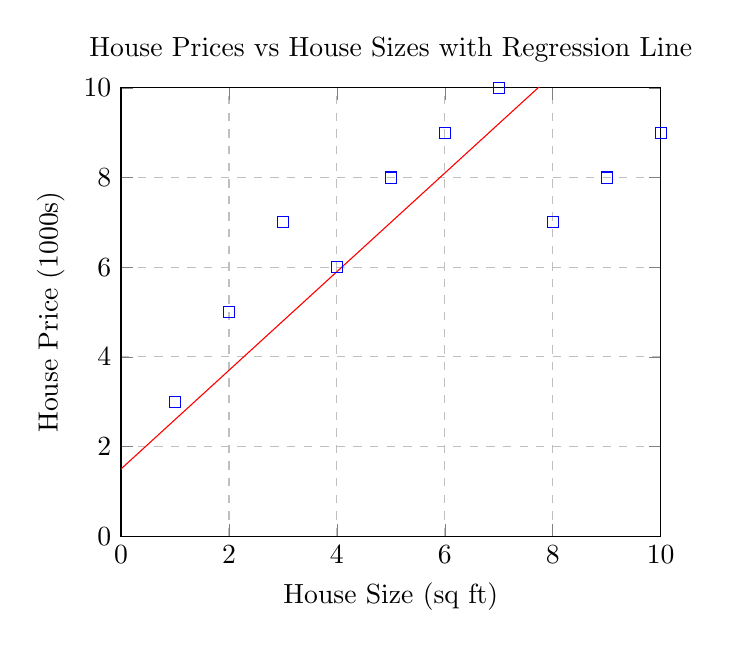
\begin{tikzpicture}
            \begin{axis}[
                title={House Prices vs House Sizes with Regression Line},
                xlabel={House Size (sq ft)},
                ylabel={House Price (1000s)},
                xmin=0, xmax=10,
                ymin=0, ymax=10,
                legend pos=north west,
                ymajorgrids=true,
                xmajorgrids=true,
                grid style=dashed,
            ]
            
            \addplot[
                only marks,
                color=blue,
                mark=square,
            ]
            coordinates {
            (1,3)
            (2,5)
            (3,7)
            (4,6)
            (5,8)
            (6,9)
            (7,10)
            (8,7)
            (9,8)
            (10,9)
            };
            
            \addplot[
                color=red,
                domain=0:10,
            ]
            {1.1*x + 1.5};
            
            \end{axis}
        \end{tikzpicture}
    \end{center}

    \paragraph*{Model Parameters (weights/coefficients)} These are the variables in the model that are learned from the training data and used to make predictions on new data. For linear regression, these parameters are \(w\) (weight or slope) and \(b\) (bias or y-intercept).

    \paragraph*{Cost Function} Also known as loss or error function, it measures the difference between the actual output and the model's predicted output, given the input. \textbf{The goal of a machine learning algorithm is to minimize the cost function}. In the context of linear regression, the cost function used is the squared error cost function, also known as Mean Squared Error (MSE). 

    Suppose that you have \(m\) examples in your training set. For each example \(i\), you have a pair of input-output \(x^i, y^i\), where \(x^i\) is the input (feature) and \(y^i\) is the actual output (label),

    You're trying to fit a linear model of the form \(f_{w,b}(x) = wx + b\), where \(w\) and \(b\) are the parameters of the model. 

    For each input \(x^i\), the model makes a prediction \(\hat{y}^i\).

    The squared error for this prediction is given by \((\hat{y}^i - y^i)^2\), which measures the square of the difference between the predicted and actual output. This squares the 'residual' or 'error' to ensure that it is positive. 

    \begin{center}
        \begin{YStkyNote}[Note]
            Is squared as it ensures that underpredictions and overpredictions are equally bad and avoids situations where they could cancel each other out.
        \end{YStkyNote}
    \end{center}

    Then, the total squared error cost is the sum of the squared errors over all \(m\) examples, given by \(\sum_{i=1}^{m}(\hat{y}^i - y^i)^2\).

    To average this over all examples,we divide by \(m\), and for mathematical convenience, we often add a division by 2, yielding the final cost function: 
    
    \[J(w,b) = \frac{1}{2m} \sum_{i=1}^{m}(\hat{y}^i - y^i)^2\]
    

    The more formal definition: 
    \[J(w,b) = \frac{1}{2m} \sum_{i=1}^{m}\left( f_{w,b}(x^i) - y^i \right)\]

    \paragraph*{3D Surface Plot} In the realm of machine learning, 3D surface plots serve as visualization tools, especially when understanding how the loss or cost function changes with respect to two parameters.

    When a model has two parameters, this optimization process can be visualized in three dimensions: two for each parameter and a third for the loss.


    \begin{center}
        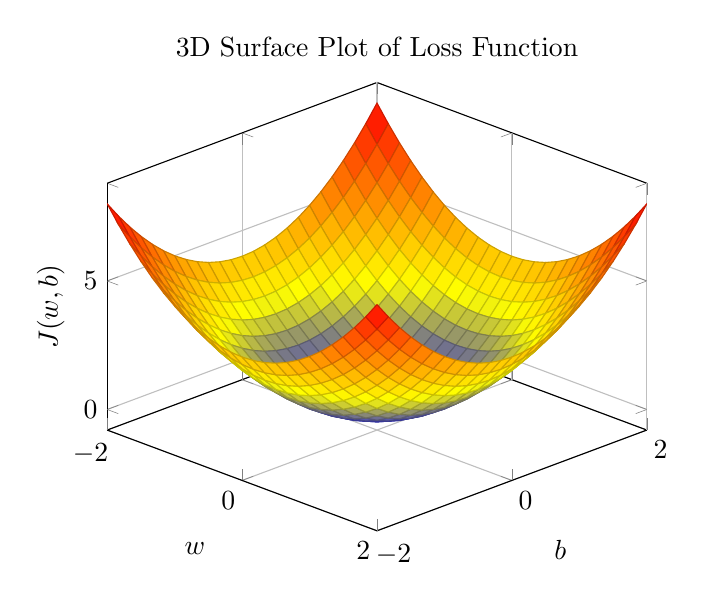
\begin{tikzpicture}
            \begin{axis}[
                title={3D Surface Plot of Loss Function},
                xlabel={\( w \)},
                ylabel={\( b \)},
                zlabel={\(J(w,b)\)},
                grid=major,
                view={45}{30} % adjust this to change your viewpoint
            ]
            \addplot3[surf, domain=-2:2, domain y=-2:2] {x^2 + y^2};
            \end{axis}
            \end{tikzpicture}
    \end{center}


    \paragraph*{Contour Plot} A contour plot provides a 2D representation of this 3D space. It's somewhat like a top-down view of the 3D plot. In a contour plot:

    \begin{itemize}
        \item Each "contour" or line represents a level curve, where the loss function has the same value.
        \item Points on the same contour have the same loss.
        \item The spacing between contours indicates the gradient or rate of change of the loss function. If the contours are closely packed, the loss function is changing rapidly.
    \end{itemize}

        

\end{document}

    % Stick Notes examples 
    % % Put the sticky note in a wrapfigure to have text wrap around it.
    % \begin{wrapfigure}{L}{0.45\textwidth}
    %     \begin{YStkyNote}[Note 1]
    %         This text is \emph{important}. Here is an useful equation:
    %         \begin{align}
    %             \sin (x) \approx x
    %         \end{align}
    %     \end{YStkyNote}
    % \end{wrapfigure}

    % \begin{wrapfigure}{R}{0.45\textwidth}
    %     \begin{PStkyNote}[Note 2]
    %     Here is some more text. This is useful information you need to know:
    %     \begin{itemize}
    %         \item sin approximation valid \textbf{only} for small angles
    %         \item 2 radians is \textit{not} a small angle
    %     \end{itemize}
    %     \end{PStkyNote}
    % \end{wrapfigure}

    % \begin{wrapfigure}{L}{0.45\textwidth}
    %     \begin{GStkyNote}[Note 3]
    %     \NB do not forget this!
    %     \end{GStkyNote}
    % \end{wrapfigure}

    % \begin{wrapfigure}{R}{0.45\textwidth}
    %     \begin{BStkyNote}[Note 4]
    %     This will be on the final exam!
    %     You better \emph{study} hard!
    %     \end{BStkyNote}
    % \end{wrapfigure}

    % \begin{wrapfigure}{L}{0.45\textwidth}
    %     \begin{WStkyNote}[Note 5]
    %         \begin{equation}
    %             pV=Nk_BT
    %         \end{equation}
    %     \end{WStkyNote}
    % \end{wrapfigure}

    % \begin{wrapfigure}{R}{0.45\textwidth}
    %     \begin{BrStkyNote}[Note 6]
    %     Type \verb+\NB+ to get the \NB text.
    %     \end{BrStkyNote}
    % \end{wrapfigure}